% !TEX root = deplump.tex
\newcommand{\T}{\ensuremath{\mathcal{T}}}
\newcommand{\N}{\ensuremath{\mathcal{N}}}
\newcommand{\M}{\ensuremath{\mathcal{M}}}
\newcommand{\PP}{\ensuremath{\mathcal{P}}}
\newcommand{\nc}{\ensuremath{nc}}
\newcommand{\RS}{\ensuremath{\mathcal{R}\mathcal{S}}}
\newcommand{\D}{\ensuremath{\mathcal{D}}}
\newcommand{\la}{\ensuremath{\leftarrow}}
\newcommand{\G}{\ensuremath{\mathcal{G}}}
\newcommand{\IS}{\ensuremath{\mathcal{I}\mathcal{S}}}
\newcommand{\Seq}{\ensuremath{\mathcal{S}}}

\begin{figure*}[t] 
	\begin{center}
		\scalebox{.6}{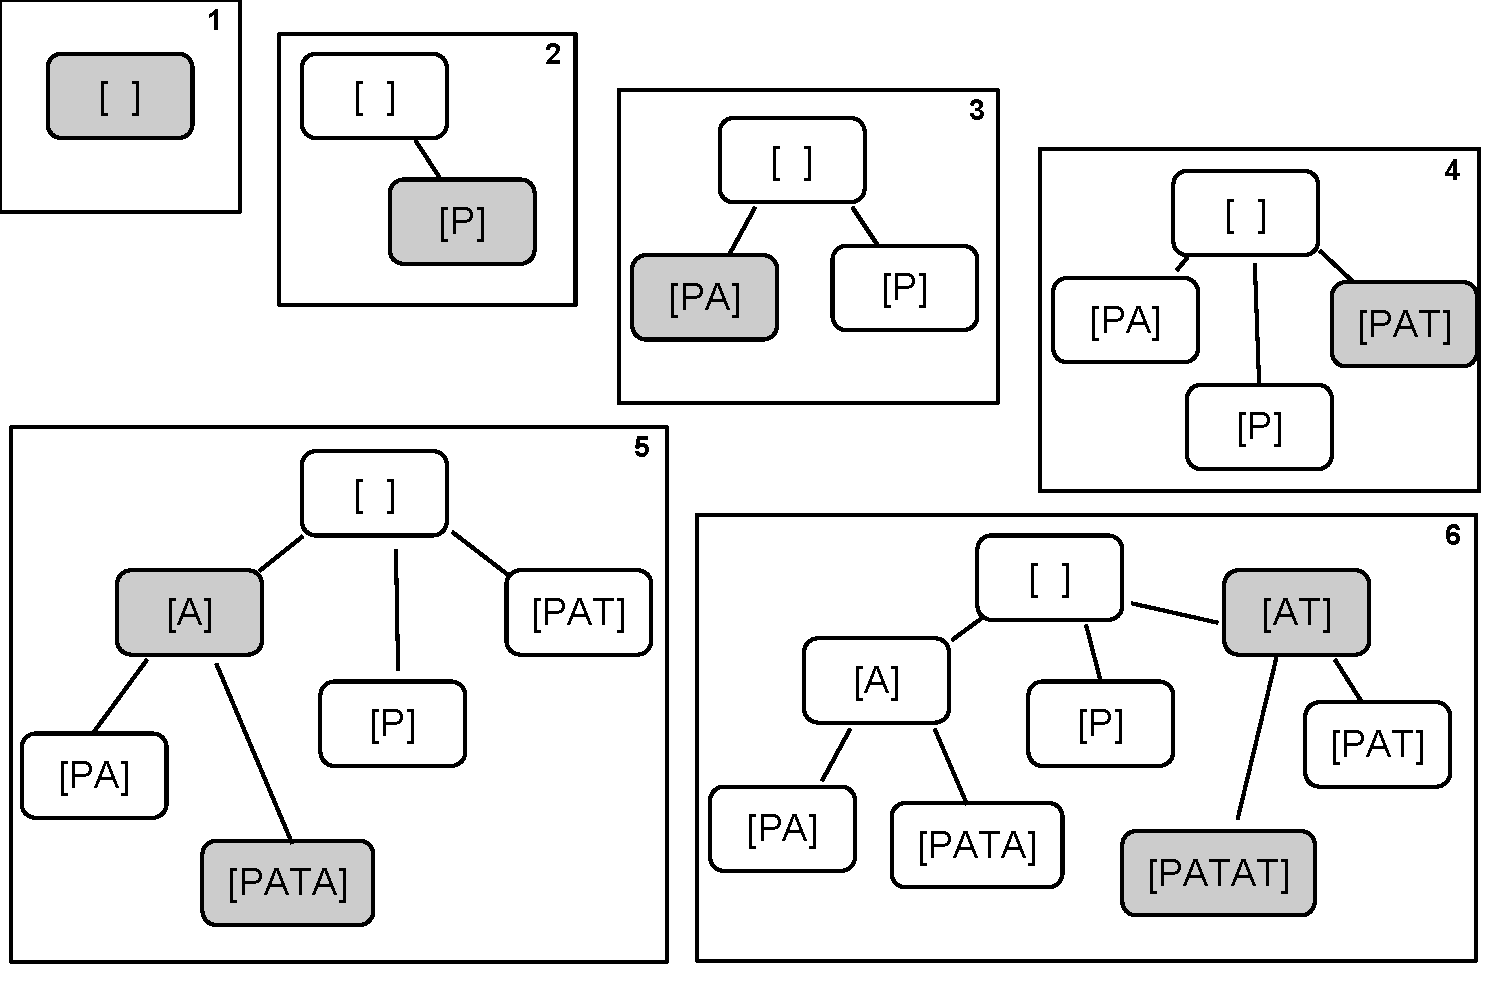
\includegraphics{PATAT.pdf}} % [clip=true, viewport= 1in 1in 9in 9in]
		\caption{Construction of suffix tree for string ``PATAT".  In each frame the new nodes are shaded in gray.}
		\label{fig:suffix_tree}
	\end{center} 
\end{figure*} 

Given an ordered symbol set $\Sigma$, probabilistic compression algorithms work by using a generative model to predict a sequence of symbols.   The predictive distribution function is then used as the parameter in a range encoder to compress the stream. The details of a range encoder implementation are not included here, we only note that if the predictive distribution function is $F$ and the next symbol in the stream is $s$ then the parameters required by the range encoder are $F(s-1)$ and $F(s)$. In the algorithm the function RangeEncode() implements the encoding and returns a bit sequence (possibly null).  The use of a cumulative distribution function is well defined since the symbols are ordered.  The notation $s-1$ refers to the symbol prior to $s$ in the symbol ordering.  In order to decompress the stream the exact same predictive model will need to be built from the compressed stream.  This requires that the model estimate prior to compressing $s_n$ is a function of fixed parameters and the symbols $[s_0, s_1, \ldots, s_{n-1}]$ because those are the only symbols available to the decompressor for decompressing $s_n$.  

The algorithm operates primarily on a suffix tree.  A suffix tree is a data structure for keeping track of unique suffices of a set of strings.  The tree structure arranges the suffices hierarchically which makes it easy to search.  In the case of a single stream the set of strings to consider is the set of contexts $\{ [ ], [s_0], [s_0,s_1], [s_0, s_1,s_2], \ldots \}$.   Each node of the suffix tree corresponds to a context of the form $[s_m, \ldots, s_{m + k}]$.  In general we will use the notation \N \space to refer interchangeably to a node object and the context to which the node corresponds. The function CreateNode($\N, \M$) makes explicit the creation of a node $\N$ associated with context $\N$ and with parent $\M$. We use the function PA(\N) to refer to the parent of node \N.

Each node object $\N$ contains two integer counts for each $s \in \Sigma$, $c_s, t_s$.  The notation $c$ and $t$ refer to the marginal counts in a node, namely $\sum_{s \in \Sigma} c_s$ and $\sum_{s \in \Sigma} t_s$.  Each node also has a discount $d$ associated with it.  The discount associated with $\N$ is a function of $\D$, the fixed discount parameters of the model, $|\N|$, and $|$PA$(\N)|$.  The function GetDiscount describes how the discount of a node $\N$ is calculated. Suffix tree data structures use a reference sequence to maintain the unique suffices in the tree.  We use the notation $\RS$ to refer to this reference sequence.  Each node $\N$ in a suffix tree contains two indices into $\RS$ from which the context specific to node $\N$ can be reconstructed.  If the indices for $\N$ are $i$ and $j$, then the context associated with $\N$ is $\RS[i : j]$.

The reference sequence $\RS$ is implemented as a linked list.  Therefore, the indexing of a suffix tree node into $\RS$ includes a pointer to a linked list node , an offset within that node and the length of the respective context.  Each node of the linked list must also contain a list of suffix tree nodes which reference it.  The reference sequence grows as the length of the compressed sequence grows and must be shortened as the algorithm progresses.  The shortening of $\RS$ is made explicit by the $\sigma$ operator in CDFNextSymbol, which returns the input sequence shortened by removing the fist element.  When $\RS$ is shortened, nodes in the suffix tree which reference removed sections are no longer usable and must be removed from the tree to prevent a memory leak.  The cost of these operations can be amortized by shorting $\RS$ in chunks by removing nodes of the linked list.  Without a list of suffix tree nodes which reference each linked list node, deletion of the unusable nodes requires a search over the tree which is prohibitive for large trees.  To minimize the impact of rendering nodes unusable by shortening the reference sequence, nodes should be updated to point to the most recent part of $\RS$ as possible.

Since the model must be estimated incrementally, the suffix tree must also be incrementally constructed.  Construction of the tree is handled by the function GetNode in Algorithm~\ref{alg}.  An illustration of the incremental construction of a suffix tree can be seen in Figure~\ref{fig:suffix_tree} for the toy sequence [PATAT].   In frame 4 the function GetNode assigns [ ]  to $\M$ and then [PAT] to $\Seq$ with $\M = $ PA$(\Seq)$. In Frame 5 GetNode assigns [PA] to $\M$, but then must assign [A] to $\PP$ with $\PP = $PA$(\M)$.  $\Seq$ is then created by CreateNode$($[PATA]$,\PP)$.  In each frame the first step is to find $\M$, which can be achieved by descending an appropriate path of the suffix tree.  All of the nodes on the path to $\M$ and possibly $\M$ itself can have the indices into $\RS$ updated to point to a later section of the reference sequence.  Finally, although not made explicit in the algorithm, it usually makes sense to limit the maximum length of a context in order to limit the depth of the suffix tree.  In Section~\ref{sec:Results} we empirically investigate performance for three values of depth.

For each $s$ in the input sequence the function CDFNextSymbol is used to obtain the predictive cumulative distribution function values of interest.  After encoding the symbol first step to updating the model estimate is performed by the function UpdateCountsAndDiscounts.  Starting at node $\N$ and progressing up to the root of the tree, $c_s$ is incremented if $t_s$ was incremented in the node below.  If $c_s$ is incremented, a stochastic decision is made to increment $t_s$.  The gradients for the discount parameters $\D$ are updated by the function UpdateDiscountParameterGradients.  Finally, if $c$ is larger than $k$ in any of the nodes, the counts $c_s$ and potentially $t_s$ are reduced by the function ThinCounts.  The parameter $k$ is a fixed parameter of the model.

First, $c_s$ is incremented in node $\N$.  A

to the root a stochastic decision is made to increment $c_s$ 


Things to make sure to include

Assumed ordering of the symols in the symbol set.
Describe paremetrization of discounts
Mention learning rate $\eta$
Describe RangeEncode function and return
Describe $\sigma$ operator
Describe size of tree $L$
Describe length of \RS \space 
Describe the deletion of leaf nodes uniformly at random
Describe pa(\N) operator
Desribe count notation
Describe CreateNode function
Mention arrays indexed from 0
Describe Draw multinomial
Discribe k in thin counts

\begin{algorithm}
    \caption{Deplump} \label{alg}
    \begin{algorithmic}[1]
    
    	\Procedure{Deplump/Plump}{$\IS , k$}
		\State $\RS \la [$ $]  $ \Comment{reference sequence}
		\State Initialize $[$ $]$ node of \T \Comment{suffix tree}
		\State $\nc \la 1$ \Comment{node count}
		\State $\D \la  \{ d_0, d_1, d_2, \dots, d_{10}, \alpha \}$ \Comment{discount parameters}
		\State $\G \la \vec 0$ \Comment{discount parameter gradients, $|\G| = |\D|$}
		\State $\mathcal{O}\mathcal{S} \la  [$ $]$ \Comment{output sequence}
		\If{Plump}
			\State $h \la $ InitializePointOnCDF(\IS)
		\EndIf
		\For{i = 0: $| \IS|$}
			\If{Plump}
				\State $[h, s, F(s-1), F(s)] \la $PointOnCDFNextSymbol$(h,\T,\RS)$
				\State $b \la s$
			\Else
				\State $s = \IS[i]$
				\State $[F(s-1), F(s)] \la $ CDFNextSymbol($s_i,\T,\RS$)
				\State $b \la$ RangeEncode$(F(s-1), F(s))$
			\EndIf
			
			\State $\mathcal{O}\mathcal{S} \la [\mathcal{O}\mathcal{S}$ $b]$ \Comment{append b to output sequence}
			\State $\D \la \D + \G \eta / (F(s) - F(s-1))$ \Comment{update discount parameters}
			\State $\G \la \vec 0$ \Comment{reset gradients to zero}
			\State $\RS \la [\RS$ $s_i]$ \Comment{append symbol to reference sequence}
		\EndFor
		\State \Return $\mathcal{O}\mathcal{S}$
	\EndProcedure
	
    	\Function{CDFNextSymbol}{$s,\T,\RS$}	
		\While{$ |\RS| \geq 100 L$}
			\State Delete nodes referencing \RS[0]
			\State $\RS \la \sigma(\RS)$
		\EndWhile
		\While{ $\nc > (L - 2)$}
			\State Delete leaf node uniformly at random
		\EndWhile
		
		\State $\N \la$ GetNode$(\RS, \T)$
		\State $\pi \la$ PMF($s, \N, \vec 0, 1.0$) \Comment{$| \vec 0| = | \Sigma|$}
		\State $F(s-1) \la \Sigma_{i = 1}^{s-1} \pi_i$
		\State $F(s) \la  F(s-1) + \pi_s$
		\State UpdateCountsAndDiscountGradients($\N,s,F(s) - F(s-1),$TRUE)
		\State \Return [$F(s-1), F(s)$]
	\EndFunction
	

	
	 \end{algorithmic}
\end{algorithm}

\begin{algorithm}
    \caption{Deplump Continued}
    \begin{algorithmic}[1]
    
    	\Function{PointOnCDFNextSymbol}{$h,\T,\RS$}
		\While{$ |\RS| \geq 100 L$}
			\State Delete nodes referencing \RS[0]
			\State $\RS \la \sigma(\RS)$
		\EndWhile
		\While{ $\nc > (L - 2)$}
			\State Delete leaf node uniformly at random
		\EndWhile

		\State $\N \la$ GetNode$(\RS, \T)$
		\State $\pi \la$ PMF($\N, \vec 0, 1.0$) \Comment{$| \vec 0| = | \Sigma|$}
		
		\State $F(s) \la 0$
		\State $s \la 0$
		\While{$F(s) < h$}
			\State $i \la i + 1$
			\State $F(s) \la F(s) + \pi_s$
		\EndWhile
		
		\State $F(s-1) \la F(s) - \pi_s$
		\State Update $h$
		\Return  $[h,s, F(s-1), F(s)]$
	\EndFunction
	
	\Function{GetDiscount}{\N}
		\State $d = 1.0$
		\For{$i = (|$PA$(\N)| + 1): |\N|$}
			\If{$i \leq 10$}
				\State $d \la d \D[i]$ \Comment{multiply by discount parameter $i$}
			\Else
				\State $d \la d \D[10]^{\D[11]^i}$
			\EndIf
		\EndFor
		\State \Return $d$
	\EndFunction
    
    	\Function{GetNode}{\Seq, \T}
		\State Find the node \M \space in the suffix tree sharing the longest suffix with \Seq.
		\If{\M \space is a suffix of \Seq}
			\If{$\Seq = \M$}
				\State \Return \M
			\Else
				\State $\Seq \la$ CreateNode$(\Seq, \M)$
				\State \Return \Seq
			\EndIf
		\Else
			\State \PP \la \space FragmentNode(\M, \Seq)
			\State PA(\M) \la \space \PP
			\State $\Seq \la $ CreateNode$(\Seq, \PP)$
			\State \Return \Seq
		\EndIf
	\EndFunction
    
    	    \end{algorithmic}
\end{algorithm}

\begin{algorithm}
	\begin{algorithmic}[1]
	\caption{Deplump Continued}
	
	\Function{UpdateCountsAndDiscounts}{$\N, s, p$, BackOff}
		\State $d \la $ GetDiscount(\N)

		\If{$c > 0$}
			\State $pp \la (p - \frac{c_i - t_i d}{c}))(\frac{c}{t d})$
			\State $tw \la c_i	+ d(t *pp - t_i)$	
		\Else
			\State $pp \la p$
		\EndIf
		
		\If{BackOff  and $c > 0$}
			\State $c^\N_s \la c^\N_s + 1$
			\State BackOff $\la 0$
			\State BackOff $\la 1$ w.p. $pp (\frac{t^\N d}{tw})$ \Comment{w.p abbreviates ``with probability"}
			\If{BackOff}
				\State $t_s \la t_s + 1$
			 \EndIf
		\Else
			\If{BackOff}
				\State $c_s \la c_s + 1$
				\State $t_s \la t_s + 1$
			\EndIf
		\EndIf
		\State UpdateDiscountParameterGradients($t_s, t,pp, d$)
		\State UpdateCountsAndDiscounts(PA(\N), $s,pp$, BackOff)
		\State ThinCounts(\N,$k$)
	\EndFunction
		

	
	\Function{ThinCounts}{$\N, k$}
		\State $d \la$ GetDiscount$(\N)$
		\While{$\sum_{s \in \Sigma} c_s > k$}
			\State $s \la $ DrawMultinomial$(\pi(\Sigma))$ s.t. $\pi_l = \frac{c_l}{c}$
			\State $\phi \la$ SamplePartition$(c_s, t_s, d)$
			\State $i \la$ DrawMultinomial$([\frac{\phi_0}{c_s}, \frac{\phi_1}{c_s}, \ldots, \frac{\phi_{t_s -1}}{c_s} ])$
			\If{$\phi_i == 1$}
				\State $t_s \la t_s - 1$
			\EndIf
			\State $c_s \la c_s - 1$
		\EndWhile
	\EndFunction	

	
	\end{algorithmic}	
\end{algorithm}

\begin{algorithm}
	\begin{algorithmic}[1]
	\caption{Deplump Continued}

\Function{PMF}{$\N, \pi, m$}
		\State $d \la $ GetDiscount(\N)		
		\If{$c > 0$}
			\For{$i \in \Sigma$}
				\State $\pi_i \la \pi_i + m(\frac{c_i - t_i d}{c})$
			\EndFor
		\EndIf
		
		\If{PA$(\N) \neq$ null}
			\State \Return PMF(PA(\N), $\pi, d m$)
		\Else
			\State $\pi \la (1- d m)\pi + dm\mathcal{U}(\Sigma)$ \Comment{$\mathcal{U}(\Sigma)$ is the uniform distribution over $\Sigma$}
			\State \Return $\pi$
		\EndIf 
	\EndFunction
	
	\Function{FragmentNode}{$\M, \Seq$}
		\State $d^\M \la$ GetDiscount(\M)
		\State $\PP \la$ maximum overlapping suffix  of \M \space and \Seq
		\State $\PP \la $ CreateNode$(\PP,$ PA$(\M))$
		\State $d^\PP \la$ GetDiscount(\PP)
		\For{$s \in \Sigma$}
			\State $\phi \la$ SamplePartition $(c^\M_s, t^\M_s,d^\M)$
			\State $c^\PP_s \la 0$
			\State $t^\PP_s \la t^\M_s$
			\State $t^\M_s \la 0$
			\For{$i= 1 : | \phi|$}
				\State $a \la$ DrawCRP$(\phi[i],d^\M / d^\PP,-d^\M)$
				\State $t_s^\M \la t_s^\M + a$
				\State $c^\PP_s \la c^\PP_s + a$
			\EndFor
		\EndFor
		\State \Return \PP
	\EndFunction
	
		\end{algorithmic}	
\end{algorithm}

\begin{algorithm}
	\begin{algorithmic}[1]
	\caption{Deplump Continued}
	
	\Function{SamplePartition}{$c,t,d$}
		\State $M \la  t \times c$ matrix of zeros
		\State $M(t,c) \la 1.0$
		\For{$j = (c-1) : 1$}
			\For{$i = 1 : (t-1)$} 
				\State $M(i,j) \la M(i +1, j+1) + M(i,j+1)(j - id)$ 
			\EndFor
			\State $M(d,j) \la M(t,j+1)$
		\EndFor
		\State $\phi \la \vec 0$ \Comment{$|\vec 0| = t$}
		\State $\phi[1] \la 1$
		\State $k \la 1$
		\For{j = 2 : c}
			\State $M(k,j) \la M(k,j)(j-1 -k d)$
			\State $r \la 0$
			\State $r \la 1 $ w.p. $\frac{M(k+1,j)}{M(k+1,j) + M(k,j)}$
			\If{r = 1}
				\State $k \la k + 1$
				\State $\phi[k]  \la 1$
			\Else
				\State $i \la$ DrawMultinomial$([\frac{\phi[1] - d}{j-1 -kd}, \frac{\phi[2] - d}{j-1 -kd}, \ldots, \frac{\phi[k] - d}{j-1 -kd}])$
				\State $\phi[i] \la \phi[i] + 1$
			\EndIf
		\EndFor
		\State \Return $\phi$
	\EndFunction


	\Function{DrawCRP}{$n,d,c$}
		\State $t \la 1$
		\For{i = 2 : n}
			\State $r \la 0$
			\State $r  \la 1$ w.p. $\frac{td + c}{i-1 + c}$
			\State $t \la t + r$
		\EndFor
		\State \Return $t$
	\EndFunction
	
	\Function{UpdateDiscountParameterGradients}{$p\_depth, depth, t_s, c, t, pp, d, m$}
		\If{$c > 0$}
			\If{$depth = 0$}
				\State derivLogDd $\la \frac{1.0}{\D[0]}$
				\State $\G[0] \la \G[0] + (d(t * pp - t_s)$derivLogDd$ / c)  m$
			\Else
				\State $z \la p\_depth + 1$
				\While{$z \leq depth$ and $z < 10$}
					\State derivLogDd $\la \frac{1.0}{\D[z]}$
					\State $\G[z] \la \G[z] + (d(t * pp - t_s)$derivLogDd$ / c)  m$	
				\EndWhile
				
				\If{$depth \geq 10$}
					\State $a \la z - 10$
					\State $b \la depth - z + 1$
					\State $\alpha \la \D[11]$
					\State $d_{10} \la \D[10]$
					\State derivLogDd $\la \alpha^a(1 - \alpha^b) / ((1 - \alpha)  d_{10})$ 
					\State $\G[10] \la \G[10] + (d(t * pp - t_s)$derivLogDd$ / c)  m$	
					\State derivLogDa $\la$ log$(d_{10}) (a \alpha^{a-1} - (a + b)\alpha^{a + b-1}) / (1 - \alpha) $
					\State \hspace{4cm} $+ (\alpha^a - \alpha^{a + b}) / (1 - \alpha)^2$
					\State $\G[11] \la \G[11] + (d(t * pp - t_s)$derivLogDa$ / c)  m$	
				\EndIf
				
			\EndIf
			
		\EndIf
	\EndFunction

	
		\end{algorithmic}	
\end{algorithm}

